\begin{appendix}

%%%%%%%%%%%%%%%%%%%%%%%%%%%%%%%%%%%%%%%%%%%%%%%%%%%%%%%%%%55
% Core size and density from Portegeis-Zwart 2010
\section{Supplemental material}

\begin{table*}
    \centering
    \caption{The age and observable stellar densities for a selection of young massive clusters found both in and outside the Milky Way, as listed in \citet{portegies2010}. Only clusters from \citet{portegies2010} which have a defined core radius, r$_c$, are shown. The densities have been calculated to only include stars which are brighter than Ks=28\m, as fainter stars will not be detectable by MICADO. The table list the parameters for the clusters shown in Fig. \ref{fig:star_density_vs_age}.}
    \label{tbl:pz10_selection}
    \begin{tabular}{l l r r r r r r}
        \hline\hline
        Galaxy & Cluster      & Distance & Age  & log(Mass) & Core radius & log$_{10}$($\rho$)    & Limiting mass \\
               &              & kpc      & Myr  & \msun     & arcsec  & stars arcsec\h{-2} & \msun         \\
        \hline
        \multicolumn{8}{c}{Cores resolvable by HST}                                                     \\
        \hline
        MW     & ONC          & 0.4      & 1    & 3.7       & 100     & -1.6           & 0.01          \\
        \hline
        \multicolumn{8}{c}{Cores resolvable by JWST}                                                    \\
        \hline
        MW     & Trumpler-14  & 2.7      & 2    & 4         & 10.7    & 1.1            & 0.01          \\
        MW     & Quintuplet   & 8.5      & 4    & 4.0       & 24      & 1.1            & 0.04          \\
        MW     & NGC3603      & 3.6      & 2    & 4.1       & 8.6     & 1.2            & 0.01          \\
        MW     & Westerlund-1 & 5.2      & 3.5  & 4.5       & 15.9    & 1.7            & 0.01          \\
        LMC    & NGC2214      & 50       & 39.8 & 4.0       & 7.5     & 1.9            & 0.1           \\
        \hline
        \multicolumn{8}{c}{Cores resolvable by MICADO}                                                  \\
        \hline
        LMC    & NGC1847      & 50       & 26.3 & 4.4       & 7.1     & 2.2            & 0.1           \\
        LMC    & NGC2157      & 50       & 39.8 & 4.3       & 8.2     & 2.2            & 0.1           \\
        LMC    & NGC1711      & 50       & 50.1 & 4.2       & 7.9     & 2.2            & 0.1           \\
        LMC    & NGC1818      & 50       & 25.1 & 4.4       & 8.5     & 2.3            & 0.1           \\
        LMC    & NGC2164      & 50       & 50.1 & 4.2       & 6.1     & 2.3            & 0.1           \\
        SMC    & NGC330       & 63       & 25.1 & 4.6       & 7.7     & 2.4            & 0.15          \\
        LMC    & NGC2136      & 50       & 100  & 4.3       & 6.6     & 2.4            & 0.1           \\
        MW     & Arches       & 8.5      & 2    & 4.3       & 4.9     & 2.5            & 0.04          \\
        LMC    & NGC1850      & 50       & 31.6 & 4.9       & 11      & 2.5            & 0.1           \\
        LMC    & NGC2004      & 50       & 20   & 4.4       & 5.8     & 2.5            & 0.1           \\
        LMC    & NGC2100      & 50       & 15.8 & 4.4       & 4.1     & 2.7            & 0.1           \\
        M31    & B257D        & 780      & 79.4 & 4.5       & 0.8     & 3.4            & 0.9           \\
        \hline
        \multicolumn{8}{c}{Only outer regions resolvable by MICADO}                                    \\
        \hline
        LMC    & R136         & 50       & 3    & 4.8       & 0.41    & 3.7            & 0.1           \\
        M31    & B066         & 780      & 70.8 & 4.3       & 0.10    & 4.2            & 0.9           \\
        M31    & B040         & 780      & 79.4 & 4.5       & 0.15    & 4.3            & 0.9           \\
        M31    & B043         & 780      & 79.4 & 4.4       & 0.19    & 4.3            & 0.9           \\
        M31    & B318         & 780      & 70.8 & 4.4       & 0.05    & 4.4            & 0.9           \\
        M31    & B448         & 780      & 79.4 & 4.4       & 0.05    & 4.4            & 0.9           \\
        M31    & Vdb0         & 780      & 25.1 & 4.9       & 0.37    & 4.4            & 0.9           \\
        M31    & B327         & 780      & 50.1 & 4.4       & 0.05    & 4.5            & 0.9           \\
        M31    & B015D        & 780      & 70.8 & 4.8       & 0.06    & 4.6            & 0.9           \\
        \hline
    \end{tabular}
\end{table*}


%%%%%%%%%%%%%%%%%%%%%%%%%%%%%%%%%%%%%%%%%%%%%%%%%%%%%%%%%%%%%%%%%%%%%%%%%%%%%%%%
% References for the cumulative cluster numbers within 2 Mpc

\begin{table*}
    \centering
    \caption{References for the cumulative cluster numbers within a 2 Mpc radius
    which will be observable by MICADO at the ELT. Star formation rate estimates 
    are based on the integrated galaxy $H_{\alpha}$ fluxes from \citet{karachentsev2013}
    and were used to estimate the true number of open clusters contained in each
    galaxy. The Milky Way clusters were taken from the HEASARC Milky Way Star Cluster
    catalogue \citep{heasarc_mwsc} and filtered to only include clusters visible to 
    MICADO at the ELT (i.e. Dec $<$ +35 deg).
    }
    \label{tbl:cum_cluster_refs}
    \begin{tabular}{lrrrl}
    
    \hline
    \hline
    Name     & SFR                  & Distance  & N Clusters & Reference      \\
             & [M$_\odot$ / yr]     & [kpc]     &            &                \\
    \hline
    MilkyWay &                      & 8         & 590        & Kharchenko+13  \\
    LMC      & 0.30                 & 50        & 456        & Glatt+10       \\
    SMC      & 0.05                 & 63        & 71         & Glatt+10       \\
    NGC6822  & 0.01                 & 499       & 24         & Karampelas+09  \\
    M33      & 0.36                 & 847       & 208        & Fan+14         \\
    NGC0055  & 0.45                 & 2128      & 168        & Castro+08      \\
    NGC0300  & 0.18                 & 2148      & 117        & Pietrzynski+01 \\
    NGC4214  & 0.15                 & 2938      & 52         & Andrews+13     \\
    \hline
    \end{tabular}
\end{table*}





%Figures A\ref{fig:results_lmc_1E3} and A\ref{fig:results_lmc_1E4} show the results for two of the 42 simulated observations. Both figures show the case of a cluster located at the distance of the LMC. In each figure the observation of the cluster can be seen along side the residuals of the subtraction process. For clusters with densities lower than 10\h3 stars arcsec\h{-2} the subtraction process worked very well, with almost all stars being accurately removed (see Fig A\ref{fig:results_lmc_1E3}). After this level the effectiveness of the PSF subtraction continually degraded with increasing density. This was to be expected. Figure A\ref{fig:results_lmc_1E4} shows the case for a 10\h4 stars arcsec\h{-2} cluster. Although the majority of stars were removed from the image, the stars which failed the fitting test remain. This was often due to two sufficiently bright stars being too close together and the fitting algorithm was not able to match a symmetrical Gaussian profile to the pair. These failed subtractions had a knock-on effect where the fainter artefacts of the PSF were detected as stars with lower signal to noise ratios, which increased the number of fake source detections. The bottom right panels Figures A\ref{fig:results_lmc_1E3} and A\ref{fig:results_lmc_1E4} shows the ratio of real mass to detected mass for each of the stars extracted from the simulated images, as well as the standard deviation for the mass ratio bins. It can be seen that the standard deviation is a good indicator for extraction reliability.


\begin{figure*}
    \centering
    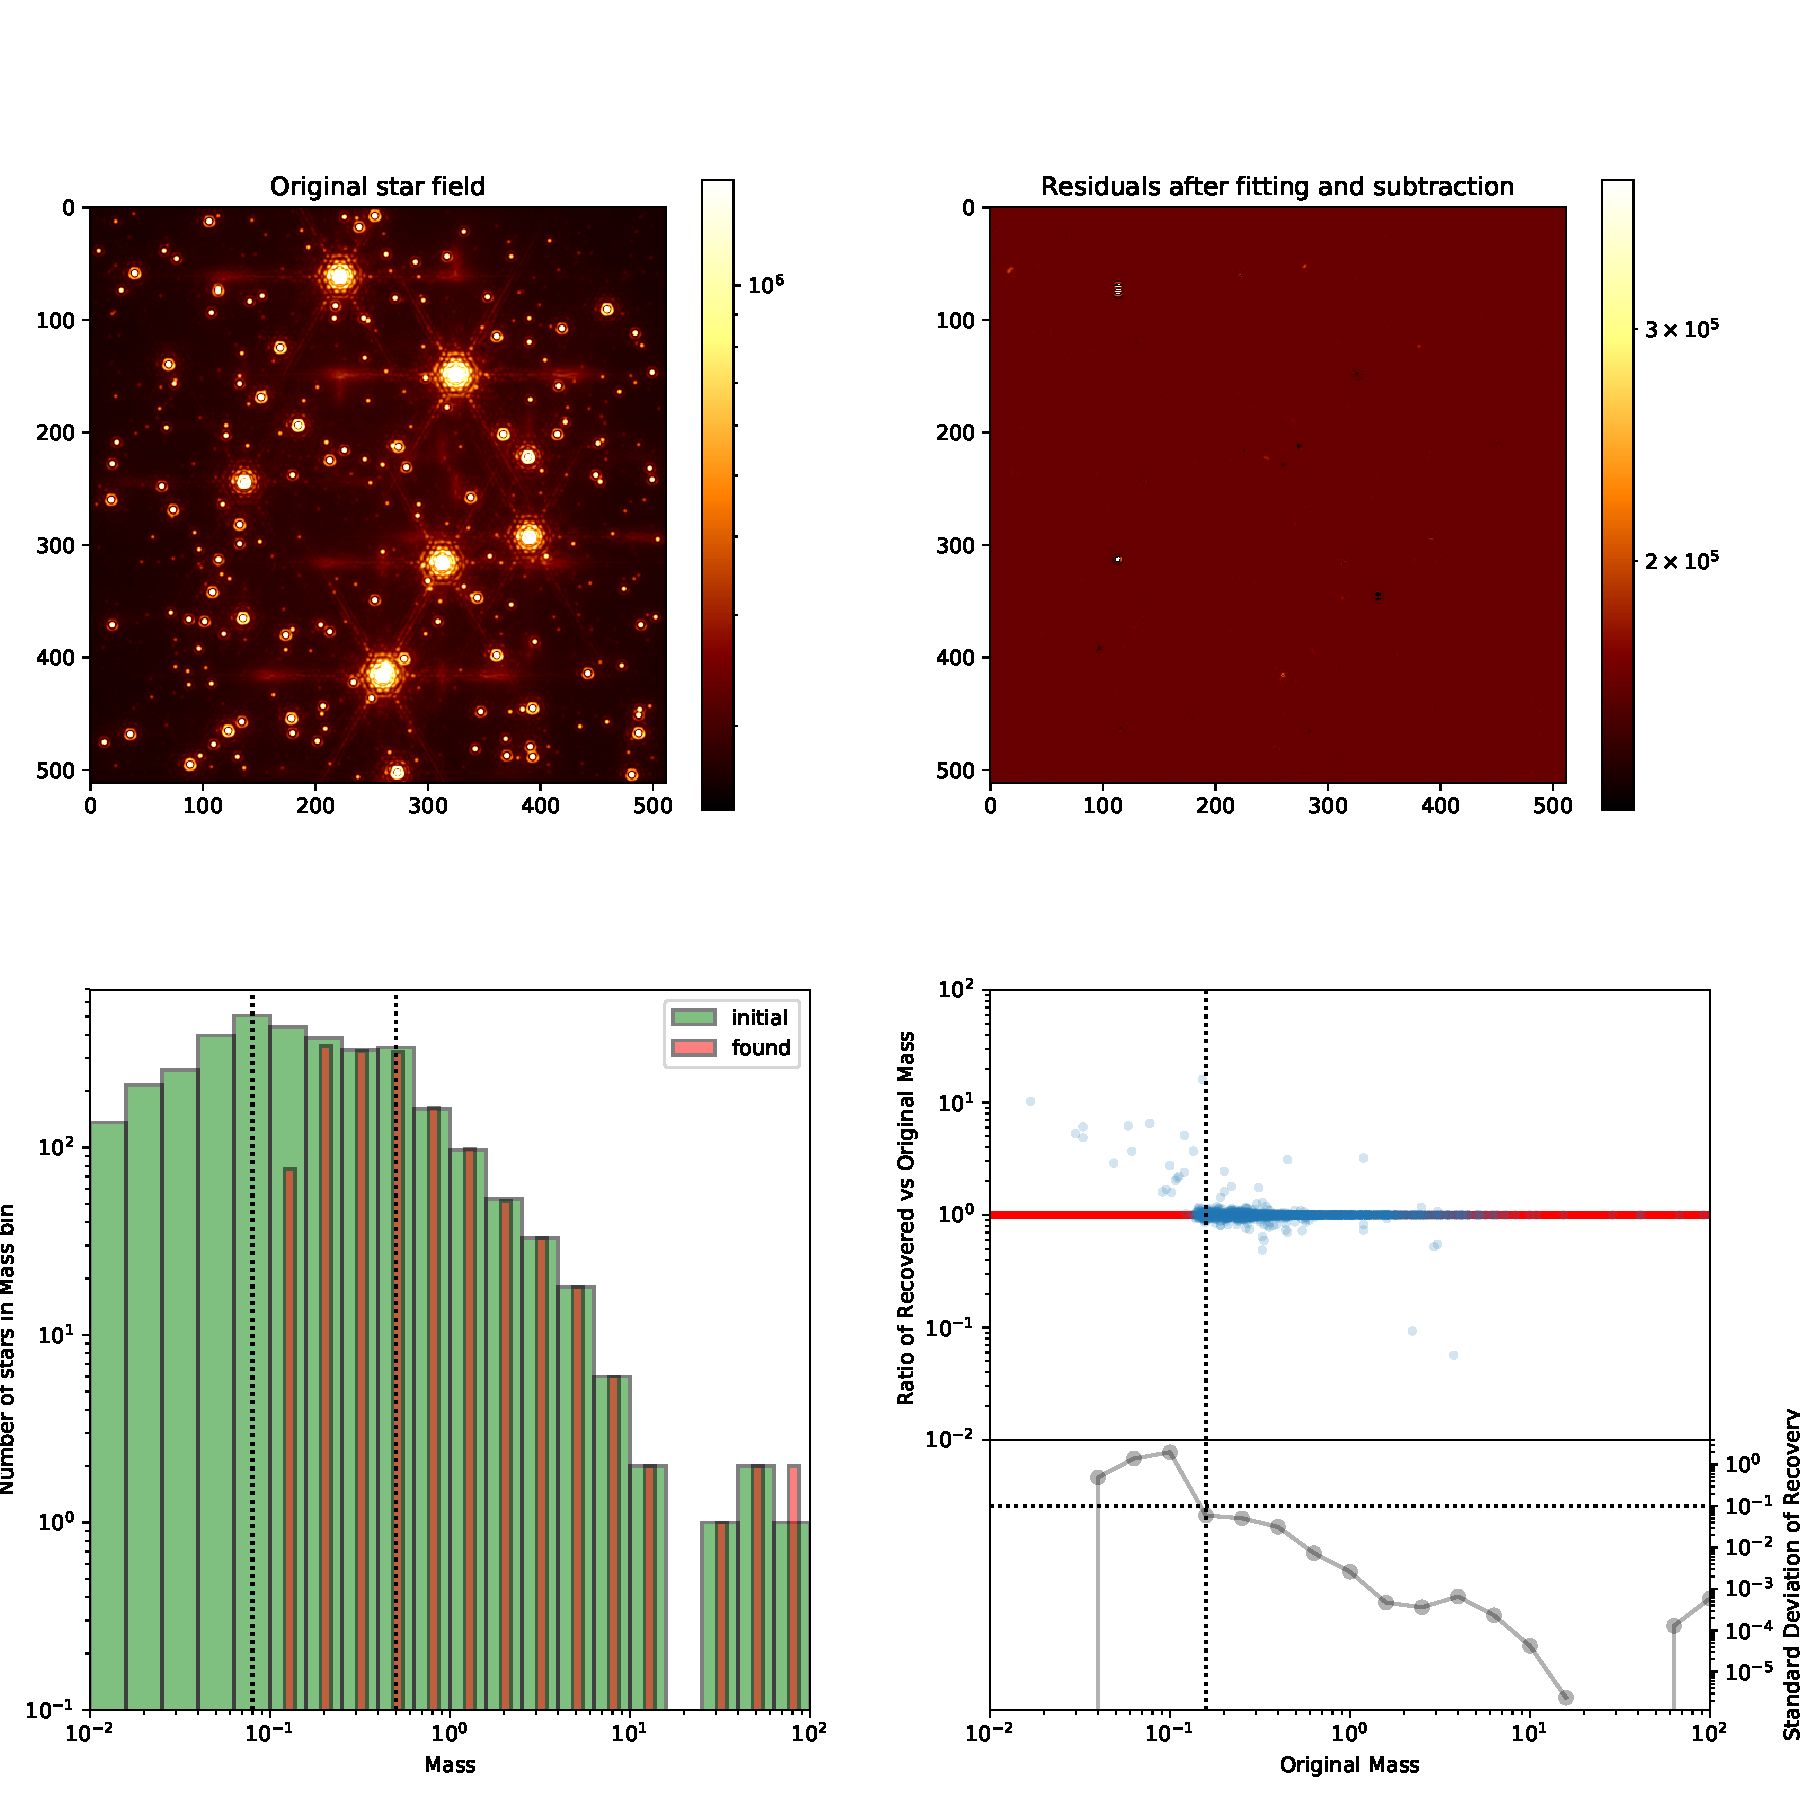
\includegraphics[width=\textwidth]{images/tbl_stats_dist=50000_rho=1000.pdf}
    \caption{Results of extracting stars from a 1000\,\spa cluster at a distance of 50\,kpc. Top left: The original 2''$\times$2'' stellar field with a density of 10\h3~\spa. The stars in the field have masses between 0.01\,\msun and 300\,\msune. The PSF used in this study was an instantaneous SCAO PSF, similar to what would be seen on a single MICADO detector 2.6\,s exposure. Top right: The same field after our detection and subtraction algorithm has iteratively removed all the stars. 10\h3~\spa are extracted reasonably easily by our algorithm. Bottom left: The fraction of extracted stars in each mass bin which matched up with the original list of stars. The majority of stars more massive than 0.1\,\msun were detected. Bottom right: The upper panel shows the ratio of extracted mass to original mass. The vast majority (\s97\%) of the almost 4000 stars in the image fell almost perfectly on the red one-to-one line. The minor scatter around the line is due to a combination of our detection algorithm not being able to discern between to very close stars, and contamination for the PSF artefacts, e.g. the segmented diffraction spikes. The lower panel shows the standard deviation of masses around the one-to-one line in a certain mass bin. A mass bin was deemed reliable if the average recovered to original mass ratio was in the range 1$\pm$0.1 and the standard deviation was less than 10\%.}
    \label{fig:results_lmc_1E3}
\end{figure*}


\begin{figure*}

    \centering
    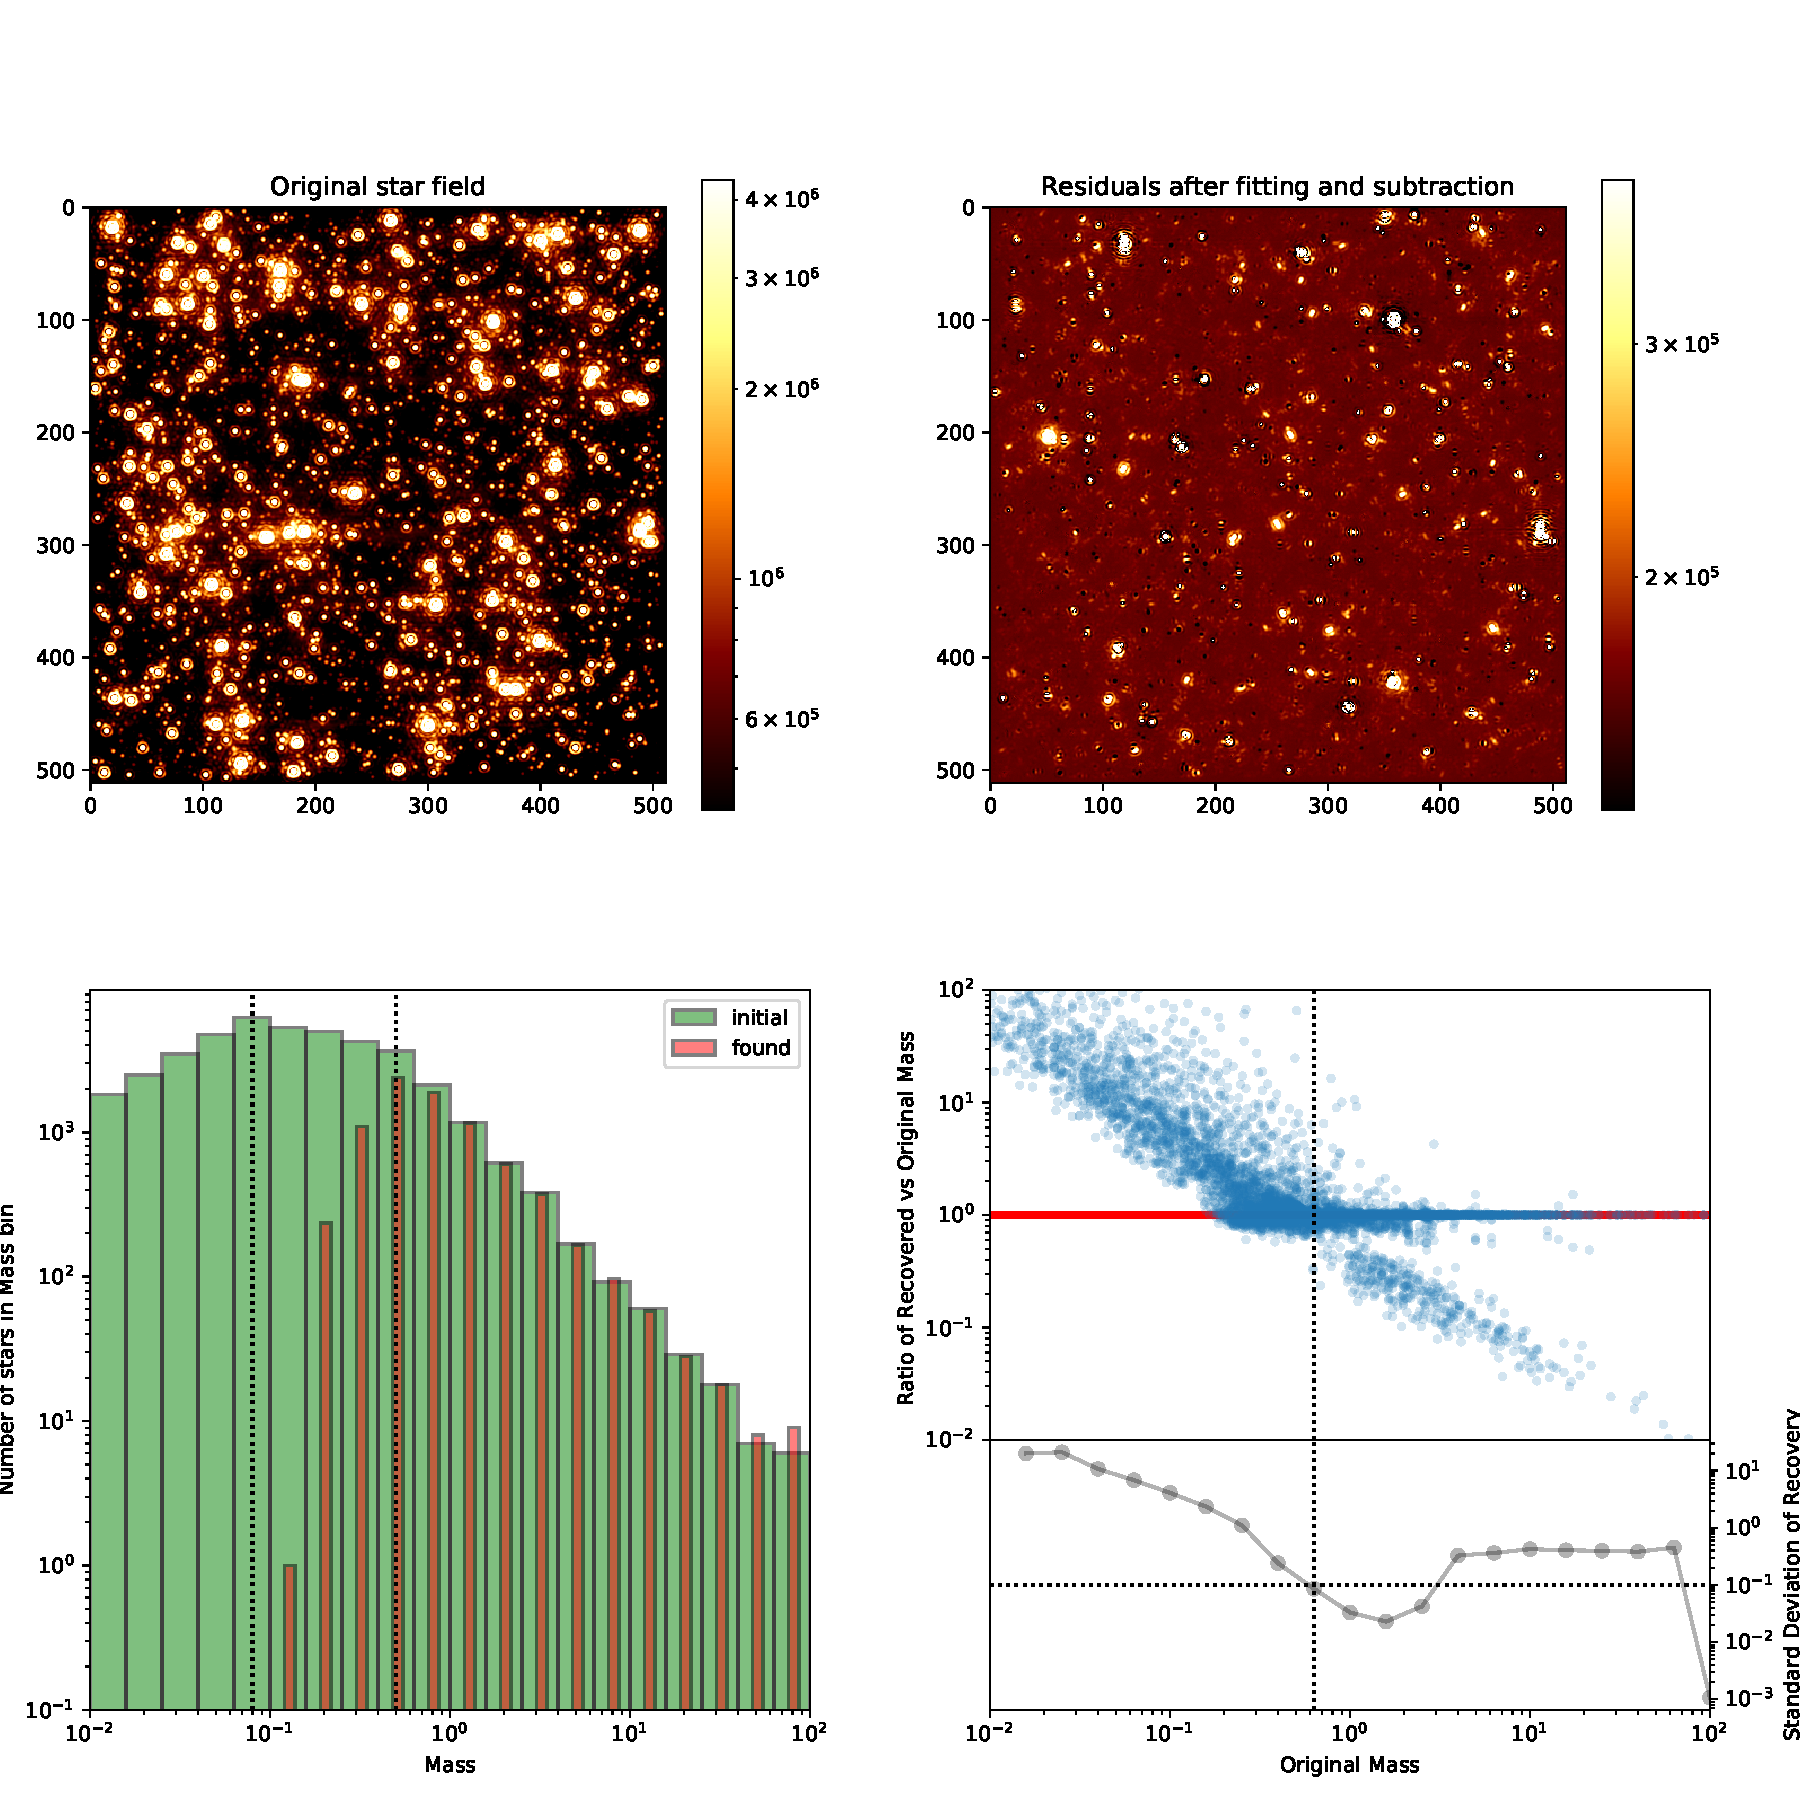
\includegraphics[width=\textwidth]{images/tbl_stats_dist=50000_rho=10000.pdf}
    \caption{Same as Fig. \ref{fig:results_lmc_1E3} but for a stellar density of 10\h4~\spa. At these densities the number of ``double'' stars has increased to the point where our detection algorithm was unable to accurately fit and subtract many of the bright stars. Although a large number of incorrect mass determinations are visible in the big blue cloud, still around 60\% of the \s40\,000 sources in this image fall on the red one-to-one line. The segmented PSF meant that the the algorithm detected many fake sources which skewed the detection statistics in both the high and low mass regimes. We are still looking into ways of preventing this from happening in future studies.}
    
    \label{fig:results_lmc_1E4}
    
\end{figure*}

\end{appendix}

